\section{Scale}\label{sec:sca}
% src: L4 (all); R1 to R3 (dennis2026communicating); B3 Sections 1, 2, 5; B5 Section 1; B1-P3, B1-P6; L6-P5, L6-P8, L6-F14, L6-F16; L7-M12, L7-P2 to L7-P4, L7-C1; critic V9 to V11, C3, D7; C2 repairs for sca

Hypothesis H4 says that the informational correlation length and time grow with the scale of collectives: media that carry messages farther, such as the telephone, or keep them longer, such as archives and international organizations, support larger and longer-lived collectives. This section turns that sentence into statements with hypotheses. It defines the correlation length $\xi$ and the correlation time $\tau$; the second-moment length $\xi_2$, contrast and the largest extent $\Lstar$ come from \cref{sec:col}. Every statement concerns world-conditional errors, because a shared world correlates all agents whether or not they communicate (Supplement, \cref{prop:sca-world-conditioning}).

The results fall into two classes. Light cones need only locality: under any local rule, attention chosen by expected free energy included, influence travels at most one hop per round, and agents more than $2t$ hops apart are independent after $t$ rounds. Every length, time and volume needs the moment bound \textup{(M)} and a named contraction of the error dynamics. The agents' own attention can violate \textup{(M)} (Supplement, \cref{ex:sca-amplifying-profile}), and then only the finite-time statements of \cref{sec:sca-lightcone,sec:sca-nomoment} survive. The section ends with H4 in final form (\cref{thm:sca-h4}).

\subsection{Hypotheses and when they fail}\label{sec:sca-hypotheses}

Different members of the scale theory need different hypotheses, so we name them once.

\begin{assumption}[Standing setting and hypothesis labels]\label{asm:sca-standing}
Agents $i\in V$ occupy the vertices of the potential communication graph $\mathcal G=(V,\mathcal E)$, with hop distance $d(i,j)$, maximal degree $\Delta$ and hop length $\ell$. The connected part $e(t)=(e_i(t))_{i\in V}$ of the agents' errors (\cref{lem:fw-common-mode}) obeys
\begin{equation}\label{eq:sca-recursion}
e(t+1)=W(t)e(t)+\zeta(t),
\end{equation}
where $W(t)$ is the error-transfer matrix of the level-0 network (\cref{def:fw-level0}) for the attention schedule of round $t$, and the local noise $\zeta(t)$ is independent across rounds with covariance $Q^\zeta(t)$; channel noise shared by several receivers is conditioned on, as in \cref{def:col-world-conditional}. Given the world path, $e(t)$ is the fluctuation of the errors about their conditional mean, so $\Sigma(t)=\Cov(e(t))$ is their world-conditional covariance, written $\Sigma^c$ in \cref{prop:col-world-conditional}, and $\Sigma$ denotes its stationary value when one exists. Block norms are spectral norms. The hypothesis labels are the following.
\begin{itemize}
\item[\textup{(Lin)}] The schedule $(W(t))_t$ is independent of the noises and of $e(0)$: it is exogenous, or chosen from deterministic quantities such as claimed covariances.
\item[\textup{(G)}] The noises and the initial law are Gaussian.
\item[\textup{(B)}] The noise is local: $Q^\zeta(t)$ is block diagonal over agents, with blocks between $q_{\min}I$ and $qI$.
\item[\textup{(Loc)}] $W_{ij}(t)\neq0$ only if $i=j$ or $(i,j)\in\mathcal E$.
\item[\textup{(M)}] The moment bound, in two forms. Stationary form: a stationary world-conditional law of $e$ with finite second moments exists. Uniform form: the agents' errors $m_i(t)-\eta_t$ have second moments bounded uniformly in $i$ and $t$, for a schedule that may vary in time and depend on the states. Unqualified, \textup{(M)} means the stationary form.
\item[\textup{(C$_r$)}] Row-sum contraction: $\lambda=\sup_t\max_i\sum_j\Vert W_{ij}(t)\Vert<1$.
\item[\textup{(C$_{rc}$)}] $\lambda_r\lambda_c<1$, where $\lambda_r=\lambda$ and $\lambda_c$ is the analogous supremum of block column sums.
\item[\textup{(C$_\rho$)}] Spectral contraction: $W$ is time invariant and $\Vert W^k\Vert_2\le K_Af^k$ for all $k\ge0$, for some $f<1$ and $K_A\ge1$; such constants exist exactly when $\rho(W)<1$.
\item[\textup{(N)}] Normality with isotropic noise ($WW^\top=W^\top W$ and $Q^\zeta=qI$), or reversibility ($WQ^\zeta=Q^\zeta W^\top$).
\item[\textup{(TI)}] Translation invariance on $\Z^D$ or on a ring.
\item[\textup{(NN)}] $W(t)\ge0$ entrywise.
\end{itemize}
\end{assumption}
% src: B3-D1; M_spec decision 16; the uniform form of (M) is the form L7-P4 (prop:min-grounding-moment) delivers

The next lemma relates the contractions; we write $\Phi(t,s)=W(t-1)\cdots W(s)$ and $\Phi(t,t)=I$.

\begin{lemma}[Relations among the hypotheses]\label{lem:sca-relations}
\begin{enumerate}
\item[(a)] Under \textup{(Lin)}, \textup{(C$_r$)} and block-diagonal noise with blocks $\preceq qI$, $\sum_j\Vert\Phi_{ij}(t,s)\Vert\le\lambda^{t-s}$ for every schedule. If in addition the initial errors $m_k(0)-\eta_0$ are independent of the schedule and have second moments bounded uniformly in $k$, $\sup_i\Vert B^{\mathrm{mis}}_i\Vert<\infty$, the world innovation has second moments bounded uniformly in time and, where codes are mistranslated, the world is stationary with finite second moments, then \textup{(M)} holds in uniform form. \textup{(M)} holds in stationary form when $W$ and the law of $\zeta(t)$ are time invariant; under \textup{(G)} the latter means a time-invariant $Q^\zeta$. If the schedule depends on the states, the population is finite with $N$ agents, every realized $W(t)$ obeys the bound of \textup{(C$_r$)}, and the initial errors and the inputs of the error recursion (local noise, world innovation and any mistranslation term) have second moments bounded uniformly, then the row-sum bound holds pathwise and \textup{(M)} holds in uniform form, with root-mean-square errors bounded by a constant that grows like $N^{1/2}$.
\item[(b)] \textup{(C$_{rc}$)} implies $\Vert W(t)\Vert_2\le(\lambda_r\lambda_c)^{1/2}<1$ for every $t$, hence \textup{(C$_\rho$)} when $W$ is time invariant.
\item[(c)] Let $W$ be time invariant and let $W$ and $Q^\zeta\succ0$ be bounded on $\ell^2(V)$, with $\rho(W)$ the spectral radius there. Then $\rho(W)<1$ implies \textup{(M)}. On a finite population the converse holds, so \textup{(M)} holds if and only if $\rho(W)<1$. On an infinite population the converse can fail. For scalar agents on $\Z^D$ under \textup{(TI)} with a summable kernel, $Q^\zeta=qI$ and symbol $\hat W(p)=\sum_xW_{0x}e^{\mathrm ip\cdot x}$, \textup{(M)} holds if and only if
\begin{equation}\label{eq:sca-fourier-moment}
\int_{[-\pi,\pi]^D}\frac{\mathrm dp}{1-|\hat W(p)|^2}<\infty,
\end{equation}
the integrand being read as $+\infty$ where $|\hat W(p)|\ge1$, and the stationary solution $\sum_{n\ge0}W^n\zeta(t-1-n)$ then has variance $q$ times the mean of the integrand over $[-\pi,\pi]^D$. The lazy walk on $\Z^3$ with $W_{xx}=1/4$ and $W_{xy}=1/8$ for $|x-y|=1$ has $\rho(W)=1$ and satisfies \eqref{eq:sca-fourier-moment}, with variance $1.4395q$; its analogues on $\Z$ and $\Z^2$ violate \eqref{eq:sca-fourier-moment}.
\end{enumerate}
\end{lemma}
% src: B3-L1(a)-(c)
Proof in \cref{app:sca}; the lazy-walk variance is computed in \cref{chk:sca-relations}. The hypotheses hold in several classes of populations.

\begin{proposition}[Sufficient conditions]\label{prop:sca-sufficient}
\begin{enumerate}
\item[(a)] Scalar level-0 receivers. With exact code models and $0\le F\le1$, every attention schedule gives \textup{(NN)} with row sums $F(1-k^s_i(t))$ (\cref{rem:fw-convex-gains}), hence \textup{(C$_r$)} with $\lambda\le F(1-\inf_{i,t}k^s_i(t))$ when the right side is below one, for instance whenever $F<1$. Then, under the moment hypotheses of \cref{lem:sca-relations}(a), \textup{(M)} holds in uniform form for exogenous schedules and, on finite populations, for schedules that depend on the states, and in stationary form for a time-invariant schedule and noise law. \textup{(C$_{rc}$)} can fail, because a sender's column sum grows with its audience.
\item[(b)] One common rank-one code. Under the hypotheses of \cref{prop:min-common-code}(b), which include level-1 receivers that know the codes and read the senders' law headers, symmetric listening, a frozen profile at its covariance fixed point and $F=fI_K$ with $0<f<1$, \textup{(C$_\rho$)} holds with rate $f$ and with $K_A=K_{\tilde M}$, the transient constant of that proposition, hence \textup{(M)}; \textup{(C$_r$)} need not hold.
\item[(c)] Noiseless grounding. Under the hypotheses of \cref{prop:min-grounding-moment} with its contraction factor $\varpi_g<1$, again at level 1, \textup{(M)} holds in uniform form for attention that depends on the past in any way.
\item[(d)] Routing at finite precision. Under the conditions of \cref{prop:sca-routing}(d), on a finite population, the routed dynamics, linear or not, has a unique stationary law, reached at an exponential rate.
\end{enumerate}
\end{proposition}
% src: B3-P1, B3-L1(e) (rem:fw-convex-gains), L7-P2, L7-P3 (prop:min-common-code), L7-P4 (prop:min-grounding-moment), L4-P3(d)
Proof in \cref{app:sca}. Part (b) matters because \textup{(C$_r$)} fails in most random common-code instances (\cref{chk:min-common-code}), so the results that assume it come with spectral versions (Supplement, \cref{prop:sca-spectral}); \cref{sec:min} lists the further conditions for stable mean dynamics derived in \citet{dennis2026communicating}. The hypotheses can fail for the agents' own attention.

In an instance taken from \citet{dennis2026communicating}, with two level-1 receivers and sender-specific codes, the attention profile that expected free energy selects has a frozen mean map with dominant eigenvalue $\rho=1.0613$, so \textup{(M)} fails in both forms (Supplement, \cref{ex:sca-amplifying-profile}). With one common code such amplification is conjectured not to occur, under the conditions stated there; \cref{prop:min-common-code} proves two cases with a rank-one code (Supplement, \cref{conj:sca-common-code}).

\subsection{Light cones}\label{sec:sca-lightcone}

The first constraint on scale needs neither stationarity nor linearity, only that every update is local.

\begin{definition}[Local rules and influence bounds]\label{def:sca-local-rule}
A local rule updates agent $i$ from its closed neighborhood $\mathcal G[i]$, the agent and its neighbors in $\mathcal G$: $\mu_i(t+1)=\mathfrak U^{(t)}_i(\mu_{\mathcal G[i]}(t),\zeta_i(t))$, with noises $\zeta_i(t)$ independent across agents and rounds. Given the world path, and with noise shared by several receivers conditioned on, this form covers messages, attention chosen from what an agent holds, and reads of records or other written external states once these are made vertices of $\mathcal G$. A matrix $\bar J\ge0$ with $\bar J_{ik}=0$ for $k\notin\mathcal G[i]$ is an influence bound if $\Vert\partial_k\mathfrak U^{(t)}_i\Vert\le\bar J_{ik}$ for all rounds, states and noises. We write $J_{ij}(t,s)=\partial\mu_i(t)/\partial\mu_j(s)$, $g_{\mathrm{tot}}=\max_i\sum_k\bar J_{ik}$ and, for $\varphi\ge0$, $g_\varphi=\max_i\sum_k\bar J_{ik}e^{\varphi d(i,k)}$.
\end{definition}
% src: L4-D1, L4-D2 (D_ij and C renamed J_ij and J_bar, L4-D2's kappa dropped); the general rule is stated here, as Section 2 directs; the map is written mathfrak U because Upsilon_ij is the mistranslation of def:fw-translation and mathcal U names the ultrametric contrast and intervention sets elsewhere

\begin{theorem}[Light cone]\label{thm:sca-lightcone}
\begin{enumerate}
\item[(a)] For $s\le t$, $\mu_i(t)$ is a measurable function of the states $\mu_k(s)$ with $d(i,k)\le t-s$ and of the noises $\zeta_k(u)$ with $s\le u<t$ and $d(i,k)\le t-1-u$. In particular $J_{ij}(t,s)=0$ when $d(i,j)>t-s$.
\item[(b)] If the initial states $\mu_i(0)$ are world-conditionally independent across agents and independent of the noises, then $\mu_i(t)$ and $\mu_j(t)$ are world-conditionally independent whenever $d(i,j)>2t$, and $\mu_i(t+h)$ and $\mu_j(t)$ whenever $d(i,j)>2t+h$.
\item[(c)] If $\bar J$ is an influence bound, then pathwise $\Vert J_{ij}(t,s)\Vert\le(\bar J^{t-s})_{ij}$, $\sum_j\Vert J_{ij}(t,s)\Vert\le g_{\mathrm{tot}}^{t-s}$, and $\Vert J_{ij}(t,s)\Vert\le e^{-\varphi d(i,j)}g_\varphi^{t-s}$ for every $\varphi\ge0$.
\end{enumerate}
\end{theorem}
% src: R1 (dennis2026communicating), L4-P1, B3-T1(a)
Proof in \cref{app:sca}; checked on a nonlinear ring (\cref{chk:sca-lightcone}). Influence travels at most one hop, a distance $\ell$, per round, as \citet{dennis2026communicating} showed for linear updates. Part (b) gives independence, which is stronger than vanishing covariance, for every local rule; correlations need two cones to overlap, so they spread at twice the influence velocity. These are exact discrete-time counterparts of Lieb--Robinson bounds \citep{lieb1972finite,marchioro1978velocity,raz2009estimating} and of the finite speed at which correlations are generated \citep{bravyi2006lieb}. When $g_\varphi>1$ influence grows inside the cone (\cref{sec:sca-nomoment}). With independent Poisson clocks of rate $\nu$, at whose events agents apply $\mathfrak U_i$, the cone acquires an exponentially small tail.

The bound on the expected influence under such clocks is in the Supplement (\cref{prop:sca-poisson}): with $g=\max_i\sum_{k\neq i}\bar J_{ik}$ and $\bar J_{\mathrm{diag}}=\max_i\bar J_{ii}$ it decays exponentially in $t$ along $d(i,j)\ge vt$ for every $v$ above the velocity $v_{\mathrm{LR}}=\max\bigl\{0,\inf_{\varphi>0}\nu(ge^\varphi+\bar J_{\mathrm{diag}}-1)/\varphi\bigr\}$ hops per unit time.

Attention chosen by expected free energy makes the update depend on beliefs through the choice itself. Let agent $i$ have a finite policy set $\mathcal P_i$, apply $\mathfrak U_{i,\pi}$ under policy $\pi$, and draw $\pi$ from the policy posterior $q_i(\pi\mid\mu)\propto E_i(\pi)e^{-\gamma G_i(\pi;\mu)}$, with habits $E_i$, policy precision $\gamma$ and expected free energy \eqref{eq:fw-efe} evaluated at the current states, independently across agents (sampled routing), or apply $\sum_\pi q_i(\pi\mid\mu)\mathfrak U_{i,\pi}$ (averaged routing). On a convex state domain let $\bar A_{ik}$ bound $\Vert\partial_k\mathfrak U_{i,\pi}\Vert$, let $\mathrm{Lip}_{ik}$ be a Lipschitz constant of $G_i(\pi;\cdot)$ in $\mu_k$, both uniform in $\pi$, and let $\mathrm{osc}_i=\sup_\mu\max_{\pi,\pi'}\Vert\mathfrak U_{i,\pi}(\mu)-\mathfrak U_{i,\pi'}(\mu)\Vert$.

\begin{proposition}[Belief-dependent routing]\label{prop:sca-routing}
Put $\bar J_{ik}(\gamma)=\bar A_{ik}+\tfrac{\gamma}{2}\mathrm{osc}_i\mathrm{Lip}_{ik}$.
\begin{enumerate}
\item[(a)] Averaged routing moves agent $i$'s coordinate by at most $\sum_k\bar J_{ik}(\gamma)\Vert\mu_k-\mu'_k\Vert$ when the state moves from $\mu$ to $\mu'$, so \cref{thm:sca-lightcone}(c) and \cref{prop:sca-poisson} hold with $\bar J(\gamma)$ in place of $\bar J$.
\item[(b)] Sampled routing admits a coupling of two copies started at $\mu(0)$ and $\mu'(0)$ with $\E\Vert\mu_i(t)-\mu'_i(t)\Vert\le\sum_j(\bar J(\gamma)^t)_{ij}\Vert\mu_j(0)-\mu'_j(0)\Vert$ in synchronous rounds.
\item[(c)] $g(\gamma)\le g(0)+\frac{\gamma}{2}\max_i\mathrm{osc}_i\sum_{k\neq i}\mathrm{Lip}_{ik}$, and $v_{\mathrm{LR}}\le eg(\gamma)\nu$ when $\bar J_{ii}(\gamma)\le1$ for all $i$.
\item[(d)] If $g_{\mathrm{tot}}(\gamma)=\max_i\sum_k\bar J_{ik}(\gamma)<1$, the averaged dynamics is a contraction in $\max_i\Vert\cdot\Vert$, and on a finite population with a closed state domain, if every $\mathrm{osc}_i$ is finite and the one-step law of the sampled dynamics from one state, hence from every state, has a finite first moment, the sampled dynamics has a unique stationary law with finite first moment, reached at an exponential rate in the Wasserstein distance. This holds for $\gamma<\gamma_D=\min_i2(1-\sum_k\bar A_{ik})/(\mathrm{osc}_i\sum_k\mathrm{Lip}_{ik})$.
\end{enumerate}
\end{proposition}
% src: L4-P3
Proof in \cref{app:sca}; checked on 300 random instances (\cref{chk:sca-routing}). Part (d) is a contraction condition in the spirit of Dobrushin's uniqueness criterion \citep{dobrushin1968description}. The bound is attained, by a chain that shows a mechanism the linear theory misses.

In that chain each relay attends one of two sources and prefers the one that agrees with what it heard: under averaged routing influence decays geometrically below a threshold of the policy precision and the sign held at the head propagates without decay above it, and under sampled routing with message noise the routing bit has, in a computed case, a correlation length of $21.5$ hops, far beyond that of the continuous content (Supplement, \cref{ex:sca-switch-chain}). At infinite policy precision causality survives and the amplitude bound fails (Supplement, \cref{rem:sca-argmax}).

\subsection{Without the moment bound}\label{sec:sca-nomoment}

\Cref{ex:sca-amplifying-profile} shows that the moment bound can fail. The support statement of \cref{thm:sca-lightcone}(b) needs nothing; the next theorem adds magnitudes without any contraction.

\begin{theorem}[Finite-time clustering without contraction]\label{thm:sca-no-moment}
Assume \textup{(Lin)}, \textup{(B)} and \textup{(Loc)}, and initial errors independent across agents with block covariances $\preceq q_0I$. Let $\bar J_{ik}=\sup_t\Vert W_{ik}(t)\Vert$, an influence bound of the linear recursion, with $g_\varphi$ as above; it may exceed one.
\begin{enumerate}
\item[(a)] For $t\ge1$, $\varphi\ge0$ and $d=d(i,j)$,
\begin{equation}\label{eq:sca-no-moment}
\Vert\Cov(e_i(t),e_j(t))\Vert\le e^{-\varphi d}\Bigl[q\sum_{n=\lceil d/2\rceil}^{t-1}g_\varphi^{2n}+q_0g_\varphi^{2t}\one\{2t\ge d\}\Bigr],
\end{equation}
and, for a lag $h\ge0$, with $(d-h)_+=\max\{d-h,0\}$,
\begin{equation}\label{eq:sca-no-moment-lag}
\Vert\Cov(e_i(t+h),e_j(t))\Vert\le e^{-\varphi d}g_\varphi^h\Bigl[q\sum_{n=\lceil(d-h)_+/2\rceil}^{t-1}g_\varphi^{2n}+q_0g_\varphi^{2t}\one\{2t+h\ge d\}\Bigr].
\end{equation}
The bracket is that of \eqref{eq:sca-no-moment} evaluated at the distance $(d-h)_+$, because the later state $e_i(t+h)$ reads $e(t)$ on a ball of radius $h$ around $i$.
\item[(b)] The top canonical correlation of $e_i(t)$ and $e_j(t)$ is at most $\Vert\Cov(e_i(t),e_j(t))\Vert/q_{\min}$. If $g_\varphi>1$, it is at most $K_\varphi\exp(-\varphi[d-2v_\varphi t])$ with $v_\varphi=\ln g_\varphi/\varphi$ and $K_\varphi=(q/(g_\varphi^2-1)+q_0)/q_{\min}$. Hence the $\theta$-correlation radius $d_\theta(t)$, the largest $d(i,j)$ at which the top canonical correlation of $e_i(t)$ and $e_j(t)$ is at least $\theta$, satisfies
\begin{equation}\label{eq:sca-radius}
d_\theta(t)\le\min\Bigl\{2t,\inf_{\varphi}\Bigl[2v_\varphi t+\varphi^{-1}\ln\frac{K_\varphi}{\theta}\Bigr]\Bigr\},
\end{equation}
the infimum running over all $\varphi>0$ with $g_\varphi>1$.
\item[(c)] If $g_\varphi<1$ for some $\varphi>0$, the bound \eqref{eq:sca-no-moment} is uniform in $t$ and decays at the rate $\varphi+\ln(1/g_\varphi)$ per hop: the stationary clustering regime.
\end{enumerate}
\end{theorem}
% src: B3-T1(b),(c)
Proof in \cref{app:sca}; checked on rings with spectral radius up to $1.33$ (\cref{chk:sca-no-moment}). Without \textup{(M)} there is no time-independent length: by \eqref{eq:sca-radius} the correlated region has radius at most $2v_\varphi t$ plus a constant, so it grows at most at twice the Lieb--Robinson velocity $v_\varphi$ and never faster than two hops per round, while for time-invariant $W$ the variances grow at least like $q_{\min}\rho(W)^{2(t-1)}$ and at most like $g_0^{2t}$. Inside the cone a time-invariant unstable profile does something specific.

Under the hypotheses stated there, a time-invariant $W$ with a simple dominant eigenvalue $\rho>1$ has $\rho^{-2t}\Sigma(t)$ converging to a rank-one matrix, so the top canonical correlation of every pair of agents on which the unstable mode is nonzero tends to one (Supplement, \cref{prop:sca-rank-one}); when the amplification sits at one site of a stable chain, the shared mode advances at less than one hop per round and is never wider than the medium's correlation length (Supplement, \cref{prop:sca-amplifying-site}). We call such an amplifying profile a rumor; it is not a collective, because the definition of a collective includes \textup{(M)} (Supplement, \cref{rem:sca-rumors}).

\subsection{Clustering}\label{sec:sca-clustering}

Under \textup{(M)} the covariance has a decay length. We define the lengths and the time of the theory and then bound them.

\begin{definition}[Correlation length and correlation time]\label{def:sca-lengths}
Let $\Sigma$ be the stationary covariance under \textup{(M)}, or, for an exogenous schedule under \textup{(M)} in uniform form, the covariance $\Sigma(t)$ of the process started in the infinite past, with bounds required uniformly in $t$. Let $R_{ij}=\Sigma_{ii}^{-1/2}\Sigma_{ij}\Sigma_{jj}^{-1/2}$ be its standardized blocks.
\begin{enumerate}
\item[(a)] On an infinite graph the correlation length in hops is $\xi\in[0,\infty]$, defined by
\begin{equation*}
\xi^{-1}=\liminf_{n\to\infty}\Bigl(-\frac1n\ln\sup_{d(i,j)\ge n}\Vert R_{ij}\Vert\Bigr),
\end{equation*}
with $\xi=0$ when the supremum vanishes for all large $n$. The mass is $m=1/\xi$, and the physical correlation length is $\ell\xi$. For families of finite graphs, bounds on $\xi$ mean bounds uniform in $|V|$.
\item[(b)] For scalar agents on $\Z^D$ under \textup{(TI)}, the Ornstein--Zernike length in coordinate direction $d$ is $\xi_{\mathrm{OZ},d}=1/m_d$, where $m_d=-\limsup_{t\to\infty}t^{-1}\ln\sum_{x:x_d=t}\Sigma(x)$ is the decay rate of the covariance summed over hyperplanes.
\item[(c)] For time-invariant $W$ with $\rho(W)<1$, the correlation time is $\tau=-1/\ln\rho(W)$ rounds.
\end{enumerate}
\end{definition}
% src: L4-D5, B1-P3(b)

\begin{theorem}[Exponential clustering]\label{thm:sca-clustering}
Assume \textup{(Lin)}, \textup{(Loc)}, \textup{(C$_r$)} and block-diagonal local noise with blocks $\preceq qI$.
\begin{enumerate}
\item[(a)] $\Phi_{ij}(t,s)=0$ if $d(i,j)>t-s$, and $\sum_j\Vert\Phi_{ij}(t,s)\Vert\le\lambda^{t-s}$.
\item[(b)] Under the moment hypotheses of \cref{lem:sca-relations}(a), \textup{(M)} holds in uniform form, and it holds in stationary form when $W$ and the law of $\zeta(t)$ are time invariant. The covariance $\Sigma(t)=\sum_{n\ge0}\Phi(t,t-n)Q^\zeta(t-1-n)\Phi(t,t-n)^\top$ of the process started in the infinite past satisfies $\Sigma(t)\succeq Q^\zeta(t-1)$ and
\begin{equation}\label{eq:sca-clustering}
\Vert\Sigma_{ij}(t)\Vert\le\frac{q\lambda^{2\lceil d(i,j)/2\rceil}}{1-\lambda^2}\le B_\Sigma e^{-m_\Sigma d(i,j)},\qquad B_\Sigma=\frac q{1-\lambda^2},\quad m_\Sigma=\ln\frac1\lambda.
\end{equation}
\item[(c)] Started at time $s$ from a block-diagonal covariance with blocks $\preceq q_0I$, $\Cov(e(t))$ obeys the same bound plus $q_0\lambda^{2(t-s)}\one\{2(t-s)\ge d(i,j)\}$.
\item[(d)] $\Vert\Cov(e_i(t+h),e_j(t))\Vert\le q\lambda^{\max(h,d(i,j))}/(1-\lambda^2)$.
\end{enumerate}
Under \textup{(B)}, $\lambda_{\min}(\Sigma(t))\ge q_{\min}$ and $\Vert R_{ij}\Vert\le\Vert\Sigma_{ij}\Vert/q_{\min}$, so $\xi\le1/\ln(1/\lambda)$.
\end{theorem}
% src: R2 (dennis2026communicating), L4-P6; constants in the form used by thm:col-markov-bound(c) and app:coh-tension
Proof in \cref{app:sca}. This is the clustering result of \citet{dennis2026communicating}, completed with the initial-condition term and the space-time cone, in the form that \cref{thm:col-markov-bound}(c) uses. In the scalar level-0 network the leak is $\varepsilon_i=1-F+Fk^s_i$ (\cref{def:fw-level0}). The bound is ballistic: its rate $\ln(1/\lambda)\approx\varepsilon$ allows lengths of order $1/\varepsilon$, whereas the exact length on lattices is of order $\sqrt{a/\varepsilon}$ (\cref{thm:sca-oz}). Four results refine it.

They are in the Supplement, each under the hypotheses stated there. With local noise correlated across agents at length $\xi_w$ the decay rate is at least $\min(\ln(1/\lambda),1/\xi_w)$, and identical agents that sense one world without communicating have a diagonal world-conditional covariance while the unconditional correlation of their errors is the same at every distance, which is why every scale bound concerns the world-conditional law (\cref{prop:sca-world-conditioning}). Under \textup{(C$_\rho$)} in place of \textup{(C$_r$)} the covariance decays at least at the rate $\ln(1/f)$ per hop, and under \textup{(B)} $\xi\le\tau$ (\cref{prop:sca-spectral}). When $W(t)$ is dominated in block norm by $\lambda$ times a reversible stochastic matrix supported on the graph, the covariance decays at least at the rate $\vartheta\sqrt{2\ln(1/\lambda)}$ per hop for every $\vartheta\in(0,1)$, the square root characteristic of diffusion (\cref{thm:sca-diffusive}). For heterogeneous nearest-neighbor media on $\Z$ the correlation length is bracketed by the Ornstein--Zernike lengths of two homogeneous media built from the extreme leaks and weights (\cref{prop:sca-heterogeneous}).

\subsection{Ornstein--Zernike decay and the second-moment length}\label{sec:sca-oz}

On lattices with nearest-neighbor attention the covariance can be computed exactly, and it shows that the length of hypothesis H4 is diffusive. Let scalar agents occupy $\Z^D$ under \textup{(TI)} with $W_{ii}=c\ge0$ and $W_{ij}=a>0$ for nearest neighbors, so that $\lambda=c+2Da=1-\varepsilon$ with $\varepsilon>0$, and let $Q^\zeta=qI$. The symbol of $W$ is $\hat W(p)=c+2a\sum_{d=1}^D\cos p_d$ for $p\in[-\pi,\pi]^D$, and its tilted counterpart is $\psi(\boldsymbol\varphi)=c+2a\sum_{d=1}^D\cosh\varphi_d$ for $\boldsymbol\varphi\in\R^D$. For a unit vector $\mathbf u\in\R^D$ let $m(\mathbf u)=\max\{\boldsymbol\varphi\cdot\mathbf u:\psi(\boldsymbol\varphi)\le1\}$, the support function of a compact convex set that contains the origin in its interior.

\begin{theorem}[Ornstein--Zernike decay on $\Z^D$]\label{thm:sca-oz}
In this setting:
\begin{enumerate}
\item[(a)] $\Sigma=q(I-W^2)^{-1}=\tfrac q2[(I-W)^{-1}+(I+W)^{-1}]$, with symbol $\hat\Sigma(p)=q/(1-\hat W(p)^2)$.
\item[(b)] For every $\boldsymbol\varphi$ with $\psi(\boldsymbol\varphi)<1$ and every $x\in\Z^D$, $\Sigma(x)\le qe^{-\boldsymbol\varphi\cdot x}/(1-\psi(\boldsymbol\varphi)^2)$. Hence along every sequence $x\to\infty$ with $x/|x|\to\mathbf u$, $\liminf-\ln\Sigma(x)/|x|\ge m(\mathbf u)$.
\item[(c)] The covariance summed over the hyperplane $\{x_1=t\}$ equals the one-dimensional covariance of part (e) with $c$ replaced by $c+2(D-1)a$. Its decay rate is $m_1=m(\mathbf u_1)$, with $\mathbf u_1$ the first coordinate unit vector, and
\begin{equation}\label{eq:sca-oz-axis}
\cosh m_1=1+\frac{\varepsilon}{2a},\qquad m_1=2\arcsinh\sqrt{\frac{\varepsilon}{4a}}=\sqrt{\frac{\varepsilon}{a}}\Bigl(1-\frac{\varepsilon}{24a}+O(\varepsilon^2)\Bigr),
\end{equation}
in every dimension, so $\xi_{\mathrm{OZ}}=1/\arccosh(1+\varepsilon/(2a))$ in each coordinate direction.
\item[(d)] Along the diagonal $\mathbf u=(1,\dots,1)/\sqrt D$, $m(\mathbf u)=\sqrt D\arccosh(1+\varepsilon/(2Da))=\sqrt{\varepsilon/a}(1-\varepsilon/(24Da)+O(\varepsilon^2))$, so the support function is isotropic to leading order, with relative anisotropy $\tfrac{\varepsilon}{24a}(1-\tfrac1D)+O(\varepsilon^2)$.
\item[(e)] For $D=1$, with $\cosh m=1+\varepsilon/(2a)$ and $\cosh m'=(1+c)/(2a)$,
\begin{equation}\label{eq:sca-oz-1d}
\Sigma(x)=\frac{q}{4a}\Bigl[\frac{e^{-m|x|}}{\sinh m}+(-1)^x\frac{e^{-m'|x|}}{\sinh m'}\Bigr],
\end{equation}
a pure exponential with no power-law prefactor ($m'>m$ when $c>0$). On a ring of even length $N$, $e^{-m|x|}$ is replaced by $\cosh(m(N/2-|x|))/\sinh(mN/2)$, and likewise for $m'$.
\item[(f)] For fixed $c>0$, as $\varepsilon\to0$: $\Sigma(0)\sim q/(4\sqrt{a\varepsilon})$ if $D=1$; $\Sigma(0)=\frac{q}{8\pi a}\ln\frac1\varepsilon+O(1)$ if $D=2$; and $\Sigma(0)$ stays bounded if $D\ge3$.
\item[(g)] $\sum_x|x|^2\Sigma(x)=4Dqa\lambda/(1-\lambda^2)^2$ and $\sum_x\Sigma(x)=q/(1-\lambda^2)$, so the second-moment length is
\begin{equation}\label{eq:sca-xi2-exact}
\xi_2^2=\frac{\sum_x|x|^2\Sigma(x)}{2D\sum_x\Sigma(x)}=\frac{2a\lambda}{1-\lambda^2}=\frac a\varepsilon\cdot\frac{2\lambda}{1+\lambda}.
\end{equation}
\end{enumerate}
\end{theorem}
% src: R3 (dennis2026communicating), L4-T1(a),(b),(d),(e),(f),(g); C2-2 repair (cosh m = 1 + eps/(2a) with lambda = c + 2Da); L4-T1(c) moved to rem:sca-oz-form
Proof in \cref{app:sca}; checked against Lyapunov solutions, Fourier inversion and direct summation (\cref{chk:sca-oz-ring,chk:sca-oz-lattice,chk:sca-lengths}). The ring case of (e) is the third result of \citet{dennis2026communicating}, which writes the rate as $\cosh m=(1-c)/(2a)$, the same number for $D=1$ only. In physical units
\begin{equation}\label{eq:sca-xi-physical}
\ell\xi_{\mathrm{OZ}}=\frac{\ell}{2\arcsinh\sqrt{\varepsilon/(4a)}}\approx\ell\sqrt{\frac a\varepsilon},
\end{equation}
H4's formula, with $a$ the weight on messages and $\varepsilon$ the leak, grounding plus forgetting (\cref{fig:sca-oz}). Distance is hop distance when $\xi$ is a few hops, since for large $\varepsilon/a$ the set $\{\psi\le1\}$ approaches a cube and $m(\mathbf u)\approx|\mathbf u|_1\ln(\varepsilon/a)$, and it becomes Euclidean only when $\xi\gg1$, where the set approaches a ball: the geometry in which a collective lives depends on its scale (\cref{asm:int-a8}). By (f) the world-conditional on-site variance diverges as $\varepsilon\to0$ when $D\le2$ and stays bounded when $D\ge3$; it adds to the shared-error floor $Q/(\varepsilon(2-\varepsilon))$ of the common mode, which diverges in every dimension (\cref{thm:coh-grounding-tension}).

\begin{figure}[t]
  \centering
  % Figure: correlation length on the ring (W_ii=c=0.25, W_ij=a for neighbors, leak eps=1-c-2a).
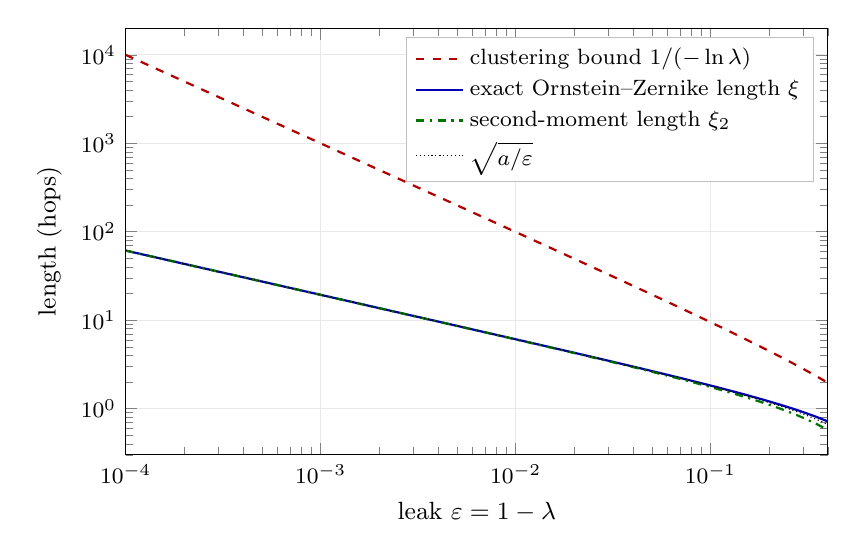
\begin{tikzpicture}
  \begin{loglogaxis}[width=10.5cm, height=7cm,
      xmin=1e-4, xmax=0.4, ymin=0.3, ymax=2e4,
      xlabel={leak $\varepsilon=1-\lambda$}, ylabel={length (hops)},
      grid=major, grid style={gray!18},
      legend style={font=\footnotesize, at={(0.98,0.98)}, anchor=north east, draw=gray!50, fill=white, cells={anchor=west}},
      every axis label/.style={font=\small}, tick label style={font=\footnotesize}]
    \addplot[red!70!black, thick, dashed] coordinates {(0.0001,9999.5) (0.000115094,8688.07) (0.000132466,7548.62) (0.00015246,6558.6) (0.000175472,5698.42) (0.000201957,4951.04) (0.00023244,4301.68) (0.000267524,3737.48) (0.000307904,3247.27) (0.000354378,2821.35) (0.000407867,2451.28) (0.00046943,2129.74) (0.000540284,1850.38) (0.000621834,1607.65) (0.000715692,1396.75) (0.000823717,1213.51) (0.000948047,1054.3) (0.00109114,915.97) (0.00125584,795.781) (0.00144539,691.354) (0.00166356,600.622) (0.00191465,521.789) (0.00220364,453.294) (0.00253625,393.782) (0.00291907,342.074) (0.00335967,297.148) (0.00386677,258.113) (0.00445041,224.198) (0.00512215,194.73) (0.00589527,169.127) (0.00678509,146.881) (0.00780922,127.553) (0.00898793,110.76) (0.0103445,96.1684) (0.0119059,83.4907) (0.013703,72.4756) (0.0157713,62.905) (0.0181518,54.5895) (0.0208916,47.3645) (0.0240449,41.0869) (0.0276742,35.6324) (0.0318512,30.8932) (0.0366588,26.7755) (0.042192,23.1976) (0.0485604,20.0888) (0.05589,17.3875) (0.0643259,15.0403) (0.0740351,13.0007) (0.0852098,11.2283) (0.0980712,9.68808) (0.112874,8.34947) (0.129911,7.186) (0.149519,6.17461) (0.172087,5.29528) (0.198062,4.53055) (0.227957,3.86526) (0.262364,3.28618) (0.301965,2.78175) (0.347543,2.34187) (0.4,1.95762)};
    \addlegendentry{clustering bound $1/(-\ln\lambda)$}
    \addplot[blue!70!black, thick] coordinates {(0.0001,61.2338) (0.000115094,57.0771) (0.000132466,53.2025) (0.00015246,49.5908) (0.000175472,46.2242) (0.000201957,43.0861) (0.00023244,40.1609) (0.000267524,37.4343) (0.000307904,34.8926) (0.000354378,32.5235) (0.000407867,30.315) (0.00046943,28.2564) (0.000540284,26.3375) (0.000621834,24.5487) (0.000715692,22.8813) (0.000823717,21.3269) (0.000948047,19.878) (0.00109114,18.5273) (0.00125584,17.2681) (0.00144539,16.0944) (0.00166356,15.0001) (0.00191465,13.98) (0.00220364,13.0291) (0.00253625,12.1425) (0.00291907,11.3159) (0.00335967,10.5452) (0.00386677,9.82667) (0.00445041,9.1567) (0.00512215,8.53198) (0.00589527,7.94944) (0.00678509,7.40618) (0.00780922,6.89952) (0.00898793,6.42696) (0.0103445,5.98617) (0.0119059,5.57495) (0.013703,5.19129) (0.0157713,4.83327) (0.0181518,4.49914) (0.0208916,4.18723) (0.0240449,3.89601) (0.0276742,3.62403) (0.0318512,3.36993) (0.0366588,3.13247) (0.042192,2.91046) (0.0485604,2.7028) (0.05589,2.50844) (0.0643259,2.32643) (0.0740351,2.15583) (0.0852098,1.9958) (0.0980712,1.8455) (0.112874,1.70417) (0.129911,1.57107) (0.149519,1.44548) (0.172087,1.3267) (0.198062,1.21405) (0.227957,1.10684) (0.262364,1.00433) (0.301965,0.905735) (0.347543,0.810157) (0.4,0.716452)};
    \addlegendentry{exact Ornstein--Zernike length $\xi$}
    \addplot[green!45!black, thick, dashdotted] coordinates {(0.0001,61.2316) (0.000115094,57.0747) (0.000132466,53.1999) (0.00015246,49.5881) (0.000175472,46.2213) (0.000201957,43.083) (0.00023244,40.1576) (0.000267524,37.4307) (0.000307904,34.8888) (0.000354378,32.5193) (0.000407867,30.3106) (0.00046943,28.2516) (0.000540284,26.3323) (0.000621834,24.5432) (0.000715692,22.8753) (0.000823717,21.3206) (0.000948047,19.8712) (0.00109114,18.52) (0.00125584,17.2603) (0.00144539,16.086) (0.00166356,14.9911) (0.00191465,13.9704) (0.00220364,13.0187) (0.00253625,12.1313) (0.00291907,11.3039) (0.00335967,10.5324) (0.00386677,9.81291) (0.00445041,9.14194) (0.00512215,8.51615) (0.00589527,7.93245) (0.00678509,7.38795) (0.00780922,6.87996) (0.00898793,6.40598) (0.0103445,5.96365) (0.0119059,5.55079) (0.013703,5.16536) (0.0157713,4.80545) (0.0181518,4.46928) (0.0208916,4.15519) (0.0240449,3.86162) (0.0276742,3.58712) (0.0318512,3.33032) (0.0366588,3.08995) (0.042192,2.86482) (0.0485604,2.65379) (0.05589,2.45583) (0.0643259,2.26993) (0.0740351,2.09516) (0.0852098,1.93062) (0.0980712,1.77549) (0.112874,1.62895) (0.129911,1.49024) (0.149519,1.3586) (0.172087,1.23331) (0.198062,1.11364) (0.227957,0.998874) (0.262364,0.888254) (0.301965,0.780986) (0.347543,0.676187) (0.4,0.572822)};
    \addlegendentry{second-moment length $\xi_2$}
    \addplot[black, densely dotted] coordinates {(0.0001,61.2332) (0.000115094,57.0764) (0.000132466,53.2017) (0.00015246,49.59) (0.000175472,46.2233) (0.000201957,43.0851) (0.00023244,40.1599) (0.000267524,37.4332) (0.000307904,34.8914) (0.000354378,32.5222) (0.000407867,30.3136) (0.00046943,28.2549) (0.000540284,26.3359) (0.000621834,24.547) (0.000715692,22.8794) (0.000823717,21.325) (0.000948047,19.8759) (0.00109114,18.525) (0.00125584,17.2657) (0.00144539,16.0918) (0.00166356,14.9974) (0.00191465,13.9771) (0.00220364,13.0259) (0.00253625,12.139) (0.00291907,11.3122) (0.00335967,10.5413) (0.00386677,9.82243) (0.00445041,9.15215) (0.00512215,8.5271) (0.00589527,7.9442) (0.00678509,7.40055) (0.00780922,6.89349) (0.00898793,6.42048) (0.0103445,5.97921) (0.0119059,5.56749) (0.013703,5.18327) (0.0157713,4.82466) (0.0181518,4.48989) (0.0208916,4.1773) (0.0240449,3.88534) (0.0276742,3.61255) (0.0318512,3.3576) (0.0366588,3.11921) (0.042192,2.89619) (0.0485604,2.68744) (0.05589,2.49191) (0.0643259,2.30861) (0.0740351,2.13662) (0.0852098,1.97507) (0.0980712,1.82312) (0.112874,1.67997) (0.129911,1.54486) (0.149519,1.41705) (0.172087,1.29581) (0.198062,1.1804) (0.227957,1.07007) (0.262364,0.964008) (0.301965,0.861317) (0.347543,0.760923) (0.4,0.661438)};
    \addlegendentry{$\sqrt{a/\varepsilon}$}
  \end{loglogaxis}
\end{tikzpicture}

  \caption{\textbf{Correlation length on the ring.} For $W_{ii}=c=0.25$ and $W_{ij}=a$ between neighbors, with leak $\varepsilon=1-c-2a$, the exact Ornstein--Zernike length $\xi_{\mathrm{OZ}}=1/\arccosh(1+\varepsilon/(2a))$ and the second-moment length $\xi_2$ both follow $\sqrt{a/\varepsilon}$, while the clustering bound of \cref{thm:sca-clustering} allows lengths up to $1/(-\ln\lambda)\approx1/\varepsilon$.}
  \label{fig:sca-oz}
\end{figure}

\Cref{thm:sca-oz} proves decay at least at the rate $m(\mathbf u)$ in every direction and exact decay of hyperplane sums. That $m(\mathbf u)$ is the exact pointwise rate, with the power-law prefactor of the Ornstein--Zernike form, follows from a theorem on walks with drift that we have read only in restatement, and the constant of the prefactor rests on a heuristic step and is not a result of this manuscript (Supplement, \cref{rem:sca-oz-form}).

The second-moment length $\xi_2$, which bounds the extent of collectives (\cref{thm:col-contrast-size}), never exceeds the Ornstein--Zernike length for translation-invariant diffusive precisions with couplings of finite range, under the hypotheses stated there, and for the medium of \cref{thm:sca-oz} $\xi_2^2\le a/\varepsilon$, so an upper bound stated with $\xi_2$ also holds there with $\xi_{\mathrm{OZ}}$ or $\sqrt{a/\varepsilon}$ (Supplement, \cref{prop:sca-lengths-relation}).

\subsection{Correlation time, diffusive scaling and records}\label{sec:sca-time}

A collective that persists must keep its variables correlated in time, and hypothesis H4 assigns that persistence to memory. The first result bounds how long any linear collective variable stays correlated; the variable may drift, since a collective is a persistent pattern and not a fixed list of coordinates (\cref{asm:int-a10}).

Under \textup{(M)} and \textup{(Lin)} with $W$ and $Q^\zeta\succ0$ time invariant, the correlation of any two linear readouts at lag $h$ is at most $\Vert\tilde W\Vert^h$ with $\tilde W=\Sigma^{-1/2}W\Sigma^{1/2}$ and $\Vert\tilde W\Vert<1$, and the lifetime $T^\ast(\theta)$, the largest lag at which some pair of readouts keeps correlation at least $\theta$, satisfies $T^\ast(\theta)/\ln(1/\theta)\to\tau$ as $\theta\to0$ (Supplement, \cref{prop:sca-persistence}). On the lattice of \cref{thm:sca-oz} time and space are tied: $\rho(W)=\lambda$ and $\xi_2^2/\tau\to a$ as $\varepsilon\to0$, so reach grows as the square root of memory and the dynamic exponent is two (Supplement, \cref{prop:sca-diffusive-scaling}).

Records lengthen memory, and we now state when. In the record model (\cref{def:fw-record-model}) the collective mean, which is the record model at wavevector zero, obeys the reduced model with transition matrix $I-\mathsf R$, where $\mathsf R$ has first row $(\varepsilon'+\sum_k\beta_k,-\beta_1,\dots,-\beta_{n_z})$, first column $(\varepsilon'+\sum_k\beta_k,-\omega_1,\dots,-\omega_{n_z})^\top$, diagonal entries $\omega_k+\delta_k$ for the records and all other entries zero, $\varepsilon'$ being the agents' leak after reading \eqref{eq:fw-record-leak}. The effective leak with records is $\varepsilon_{\mathrm{rec}}=\lambda_{\min}(\mathsf R)$, and $\mathcal R_k=\beta_k/\omega_k$ is the read-to-write ratio of record $k$.

\begin{proposition}[The secular equation]\label{prop:sca-records}
Let $\beta_k>0$, $\omega_k>0$ and $\omega_k+\delta_k>0$ for every $k$, and put
\begin{equation}\label{eq:sca-secular}
g_z(x)=\varepsilon'-x+\sum_k\beta_k\frac{\delta_k-x}{\omega_k+\delta_k-x}.
\end{equation}
\begin{enumerate}
\item[(a)] Every eigenvalue of $\mathsf R$ is real.
\item[(b)] $g_z$ is strictly decreasing on $(-\infty,\min_k(\omega_k+\delta_k))$ and has exactly one root $x_0$ there; $x_0=\varepsilon_{\mathrm{rec}}$; and $\varepsilon_{\mathrm{rec}}\ge0$ if and only if $\varepsilon'+\sum_k\beta_k\delta_k/(\omega_k+\delta_k)\ge0$.
\item[(c)] If $I-\mathsf R\ge0$ entrywise, then $\rho(I-\mathsf R)=1-\varepsilon_{\mathrm{rec}}$, and the correlation time of the mean mode is $\tau=-1/\ln(1-\varepsilon_{\mathrm{rec}})$.
\item[(d)] Let the agents-only transition matrix $W_0\ge0$ of a network have constant row sums $1-\varepsilon$, and let every agent read record $k$ with weight $\beta_k$ taken from its self-weight, while record $k$ is written with weights $\omega_{k,i}\ge0$ that sum to $\omega_k$. If the joint transition matrix of agents and records is entrywise nonnegative, its spectral radius is $1-\varepsilon_{\mathrm{rec}}$, with $\varepsilon_{\mathrm{rec}}$ from the reduced model with $\upsilon_k=0$, whatever the write weights.
\end{enumerate}
\end{proposition}
% src: B5-P1, B5-P3(a)
Proof in \cref{app:sca}; checked on 3000 random models (\cref{chk:sca-records}). Under block averaging the record equation closes exactly and the record parameters do not renormalize, and on $\Z^D$ with cubic blocks the reduced model, hence $\varepsilon_{\mathrm{rec}}$, is the same at every level (\cref{thm:ren-closure}(e)). Whether records lengthen memory is decided by the sign of one function.

\begin{proposition}[Exact memory criterion]\label{prop:sca-records-memory}
Assume \cref{prop:sca-records} and $\varepsilon_{\mathrm{rec}}\ge0$.
\begin{enumerate}
\item[(a)] Reading that displaces self-weight ($\upsilon_k=0$). The effective leak lies between the agents' leak and the record decays, $\min\{\varepsilon,\delta_1,\dots,\delta_{n_z}\}\le\varepsilon_{\mathrm{rec}}\le\max\{\varepsilon,\delta_1,\dots,\delta_{n_z}\}$, strictly for one record with $\delta\neq\varepsilon$. When $\varepsilon<\min_k(\omega_k+\delta_k)$,
\begin{equation}\label{eq:sca-memory-criterion}
\varepsilon_{\mathrm{rec}}<\varepsilon\iff\sum_k\beta_k\frac{\delta_k-\varepsilon}{\omega_k+\delta_k-\varepsilon}<0,
\end{equation}
and $\varepsilon_{\mathrm{rec}}<\varepsilon$ always when $\varepsilon\ge\min_k(\omega_k+\delta_k)$. Records lengthen the memory if every $\delta_k<\varepsilon$ and shorten it if every $\delta_k>\varepsilon$, and when $I-\mathsf R\ge0$, $\tau\le-1/\ln(1-\min\{\varepsilon,\delta_1,\dots,\delta_{n_z}\})$.
\item[(b)] One record with $\delta=0$: $\varepsilon/(1+\mathcal R+\varepsilon/\omega)\le\varepsilon_{\mathrm{rec}}\le\varepsilon/(1+\mathcal R)$, so the extension factor $\varepsilon/\varepsilon_{\mathrm{rec}}$ of the decay rate lies in $[1+\mathcal R,1+\mathcal R+\varepsilon/\omega]$. Since $\varepsilon_{\mathrm{rec}}$ increases with $\delta$, $1+\mathcal R+\varepsilon/\omega$ bounds the extension for every $\delta\ge0$.
\item[(c)] General displacement. For one record with $\upsilon<1$, $\varepsilon_{\mathrm{rec}}<\varepsilon$ if and only if $\delta<\varepsilon+\upsilon\omega/(1-\upsilon)$; with $\upsilon=1$, $\varepsilon_{\mathrm{rec}}<\varepsilon$ for every $\delta$. For several records with $\varepsilon<\min_k(\omega_k+\delta_k)$, $\varepsilon_{\mathrm{rec}}<\varepsilon$ if and only if $\sum_k\beta_k[(\delta_k-\varepsilon)/(\omega_k+\delta_k-\varepsilon)-\upsilon_k]<0$.
\item[(d)] Adding nonnegative weight to an entrywise nonnegative transition matrix never lowers its spectral radius; in particular a record with self-weight $1-\omega-\delta$ forces $\rho\ge1-\omega-\delta$. This is the endpoint $\upsilon=1$ of (c).
\item[(e)] With $\upsilon_k=0$, as $(\varepsilon,\delta_1,\dots,\delta_{n_z})\to0$ at fixed $\beta_k$ and $\omega_k$,
\begin{equation}\label{eq:sca-records-tau}
\varepsilon_{\mathrm{rec}}=\frac{\varepsilon+\sum_k\mathcal R_k\delta_k}{1+\sum_k\mathcal R_k}+O\bigl(|(\varepsilon,\delta)|^2\bigr),\qquad\tau=\frac{1+\sum_k\mathcal R_k}{\varepsilon+\sum_k\mathcal R_k\delta_k}\bigl(1+o(1)\bigr).
\end{equation}
\end{enumerate}
\end{proposition}
% src: B5-P2(a)-(e), L5-P8(b) via the secular equation; C2-10
Proof in \cref{app:sca}; checked on random draws (\cref{chk:sca-records}). A medium lengthens collective memory only if it decays more slowly than the agents forget, in the weighted sense of \eqref{eq:sca-memory-criterion}: a durable record alone can multiply $\tau$ by $4.90$, while adding a heavily read perishable record makes $\varepsilon_{\mathrm{rec}}$ exceed $\varepsilon$ (\cref{chk:sca-records}). For a level-0 receiver whose prior precision is held fixed, Kalman weights are proportional to precisions, so reading displaces the sensing weight in the proportion of the sensing gain before reading, $\upsilon=k^s$; the conservative default is $\upsilon=0$. With $\upsilon_k=0$ the leading term of (e) is an exact upper bound on $\varepsilon_{\mathrm{rec}}$ for all nonnegative leaks, with a lower bound through the weighted dispersion of the leaks, and with leaks only at the agents, nested records, records read and written by other records, lengthen memory further, with weights that are products of read-to-write ratios along the chain (\cref{prop:hie-nested-records}).

Worked special cases are in the Supplement (\cref{rem:sca-records-special}), among them the identity time of a collective whose members turn over (\cref{prop:agy-identity}), whose rate is, under the dictionary given there and when the record is read, the secular root $\varepsilon_{\mathrm{rec}}$.

Records also change the length.

\begin{proposition}[The length with records]\label{prop:sca-records-length}
Consider the record model of \cref{def:fw-record-model} on $\Z^D$ with $a>0$, $\beta_k>0$ and $\omega_k>0$, read kernels $\mathsf K_k$ invariant under permutations and reflections of the coordinates, an entrywise nonnegative transition matrix ($1-\varepsilon'-\sum_k\beta_k-2Da\ge0$ and $\omega_k+\delta_k\le1$) and $\rho(I-\mathsf R)<1$. Its symbol at wavevector $p$ is the $(1+n_z)\times(1+n_z)$ matrix $\hat{\mathsf W}(p)=\hat{\mathsf W}_0-|p|^2\mathsf R_2+o(|p|^2)$, with $\hat{\mathsf W}_0=I-\mathsf R$ and $\mathsf R_2$ the matrix whose first row is $(a,\beta_1\ell_{r,1}^2/2,\dots,\beta_{n_z}\ell_{r,n_z}^2/2)$ and whose other entries vanish, and $Q_z=\diag(q,q_z,\dots,q_z)$ holds the noise variances of the definition.
\begin{enumerate}
\item[(a)] Exact formula. Let $\Sigma_0$ and $\Sigma_2$ solve
\begin{equation}\label{eq:sca-records-lyap}
\Sigma_0=\hat{\mathsf W}_0\Sigma_0\hat{\mathsf W}_0^\top+Q_z,\qquad\Sigma_2=\hat{\mathsf W}_0\Sigma_2\hat{\mathsf W}_0^\top+\mathsf R_2\Sigma_0\hat{\mathsf W}_0^\top+\hat{\mathsf W}_0\Sigma_0\mathsf R_2^\top.
\end{equation}
Then the agents' covariance-side second-moment length is $\xi_2^2=(\Sigma_2)_{00}/(\Sigma_0)_{00}$.
\item[(b)] Asymptotics. The $|p|^2$-coefficient of the slow eigenvalue of $I-\hat{\mathsf W}(p)$, in hops squared per round, is
\begin{equation}\label{eq:sca-deff}
\mathcal D_{\mathrm{eff}}=\frac{a+\sum_k\frac{\beta_k\omega_k}{\omega_k+\delta_k-\varepsilon_{\mathrm{rec}}}\frac{\ell_{r,k}^2}{2}}{1+\sum_k\frac{\beta_k\omega_k}{(\omega_k+\delta_k-\varepsilon_{\mathrm{rec}})^2}}.
\end{equation}
For $\upsilon_k=0$, as $(\varepsilon,\delta_1,\dots,\delta_{n_z})\to0$ at fixed $a$, $\beta_k$, $\omega_k$, $\ell_{r,k}$, $q$ and $q_z$,
\begin{equation}\label{eq:sca-records-xi}
\xi_2^2=\frac{\mathcal D_{\mathrm{eff}}}{\varepsilon_{\mathrm{rec}}}\bigl(1+O(\varepsilon_{\mathrm{rec}})\bigr)=\frac{a+\sum_k\beta_k\ell_{r,k}^2/2}{\varepsilon+\sum_k\mathcal R_k\delta_k}\bigl(1+o(1)\bigr).
\end{equation}
\item[(c)] Link to the size bound. Suppose that the world-conditional precision of agents and records together is diffusive. Then so is the agents' marginal precision, with the records marginalized, the length of (a) is its second-moment length, and every region $C$ of agents whose contrast, computed from the joint precision, is at least $r_0>1$ satisfies $\Var_d(C)\le\xi_2^2/(r_0-1)$ in every coordinate.
\end{enumerate}
\end{proposition}
% src: B5-P5(a),(b),(d); C2 repair (iii): the sketched step of B5-P5(b) is replaced by a finite-dimensional argument in app:sca, checked numerically in this editing round; C2 S4 and decision 13: (c) needs diffusivity
Proof in \cref{app:sca}; checked on a ring of $2000$ sites (\cref{chk:sca-records-length}). The proof of (b) expands the two finite Lyapunov equations of (a) around the slow eigenvalue of $\mathsf R$, which stays simple and isolated as the leaks vanish. The constant in its error term carries the factor $(1+\sum_k\mathcal R_k)^2$, the inverse squared weight of the agents in the slow mode, so at finite leaks $\xi_2$ can lie well below the slow-branch value $(\mathcal D_{\mathrm{eff}}/\varepsilon_{\mathrm{rec}})^{1/2}$. To leading order, local records ($\ell_{r,k}=0$) slow a collective without widening it, leaving $\xi_2$ unchanged when $\delta_k=0$ and shortening it when $\delta_k>0$, while $\tau$ grows by the factor $(1+\sum_k\mathcal R_k)\varepsilon/(\varepsilon+\sum_k\mathcal R_k\delta_k)$; reading at range adds $\sum_k\beta_k\ell_{r,k}^2/2$ to the numerator, and $\xi_2^2/\tau\to(a+\sum_k\beta_k\ell_{r,k}^2/2)/(1+\sum_k\mathcal R_k)$. Part (c) needs its hypothesis: with record noise the agents' marginal precision had positive off-diagonal entries in a computed case, so neither it nor the joint precision is diffusive and the size bound does not apply (\cref{rem:col-which-contrast,chk:sca-records-length}). A durable noiseless global record of a closed collective of $n$ members also violates it, since the precision with the record node then has a positive entry for every pair of members coupled more weakly than $\omega/n$ (\cref{ex:hie-noiseless-record}). At the record noise that makes the dynamics reversible, that precision is diffusive and the contrast with the record as a node has a closed form (\cref{prop:hie-record-contrast}), but whether such a region is a collective needs a comparison medium for populations with record nodes, which is open (\cref{open:col-records-baseline}). \Cref{fig:sca-records} shows both effects on the ring of \cref{chk:sca-records-length}: the correlation time crosses its value without records exactly at $\delta=\varepsilon$, and the second-moment length grows with the reading range, while a local record leaves it below its value without records.

\begin{figure}[t]
  \centering
  % Figure: records on a ring with a=0.2 and eps=0.002 (record model, reading displaces self-weight, q=1, q_z=0).
% (a) tau=-1/ln(1-eps_eff), eps_eff the root of the secular equation g_z (prop:sca-records), one local record
%     with beta=0.1 and omega=0.01 or 0.1; 61 values of delta, log-spaced from 1e-5 to 0.2.
% (b) xi_2^2=(Sigma_2)_00/(Sigma_0)_00 from the two Lyapunov equations of prop:sca-records-length(a),
%     durable record (beta,omega,delta)=(0.1,0.01,1e-4); dashed: leading-order form of eq:sca-records-xi.
% Computed in double precision (Brent root of g_z, Kronecker-form Lyapunov solves). The same computation,
% with a real-space second moment on a ring of 2000 sites, reproduces every value of chk:sca-records-length
% (xi_2=9.995, 7.265, 16.308, 3.592, 22.527, 12.957; tau=499.5, 3702.5, 286.1, 211.3, 3702.5, 1381.1).
\begin{tikzpicture}
  \begin{loglogaxis}[name=pa, scale only axis, width=5.9cm, height=4.9cm, set layers,
      xmin=1e-5, xmax=0.2, ymin=5, ymax=5e4,
      xlabel={record decay $\delta$}, ylabel={correlation time $\tau$ (rounds)},
      grid=major, grid style={gray!18},
      legend style={font=\footnotesize, at={(0.035,0.045)}, anchor=south west, draw=gray!50, fill=white, cells={anchor=west}},
      every axis label/.style={font=\small}, tick label style={font=\footnotesize}]
    \begin{pgfonlayer}{axis background}
      \fill[green!7] (axis cs:1e-5,5) rectangle (axis cs:0.002,5e4);
    \end{pgfonlayer}
    % beta=0.1, omega=0.01 (R=10)
    \addplot[blue!70!black, thick] coordinates {(1e-05,5319.3) (1.1795e-05,5273.4) (1.3911e-05,5220.2) (1.6408e-05,5158.9) (1.9352e-05,5088.4) (2.2825e-05,5007.7) (2.6922e-05,4915.7) (3.1753e-05,4811.4) (3.7452e-05,4694) (4.4173e-05,4562.7) (5.21e-05,4417) (6.145e-05,4256.7) (7.2478e-05,4081.9) (8.5485e-05,3893.3) (0.00010083,3692.2) (0.00011892,3480.1) (0.00014026,3259.3) (0.00016543,3032.4) (0.00019512,2802.3) (0.00023014,2572.1) (0.00027144,2344.9) (0.00032016,2123.7) (0.00037761,1911) (0.00044538,1709.2) (0.00052531,1519.8) (0.00061958,1344.2) (0.00073077,1183) (0.00086191,1036.4) (0.0010166,904.25) (0.001199,786.05) (0.0014142,681.07) (0.001668,588.39) (0.0019674,507.03) (0.0023204,435.95) (0.0027368,374.11) (0.003228,320.5) (0.0038073,274.19) (0.0044906,234.27) (0.0052965,199.96) (0.006247,170.53) (0.0073681,145.32) (0.0086903,123.77) (0.01025,105.37) (0.012089,89.674) (0.014259,76.301) (0.016818,64.919) (0.019836,55.24) (0.023396,47.019) (0.027595,40.043) (0.032547,34.133) (0.038388,29.137) (0.045277,24.928) (0.053402,21.4) (0.062986,18.47) (0.074289,16.077) (0.087622,14.176) (0.10335,12.731) (0.12189,11.693) (0.14377,10.984) (0.16957,10.512) (0.2,10.196)};
    \addlegendentry{$\omega=0.01$}
    % beta=0.1, omega=0.1 (R=1)
    \addplot[red!70!black, thick, dashed] coordinates {(1e-05,999.45) (1.1795e-05,998.54) (1.3911e-05,997.48) (1.6408e-05,996.22) (1.9352e-05,994.75) (2.2825e-05,993.02) (2.6922e-05,990.98) (3.1753e-05,988.59) (3.7452e-05,985.78) (4.4173e-05,982.49) (5.21e-05,978.64) (6.145e-05,974.13) (7.2478e-05,968.87) (8.5485e-05,962.74) (0.00010083,955.61) (0.00011892,947.33) (0.00014026,937.76) (0.00016543,926.7) (0.00019512,914) (0.00023014,899.46) (0.00027144,882.9) (0.00032016,864.14) (0.00037761,843.01) (0.00044538,819.4) (0.00052531,793.19) (0.00061958,764.37) (0.00073077,732.98) (0.00086191,699.12) (0.0010166,663.03) (0.001199,625) (0.0014142,585.43) (0.001668,544.8) (0.0019674,503.61) (0.0023204,462.45) (0.0027368,421.84) (0.003228,382.33) (0.0038073,344.38) (0.0044906,308.38) (0.0052965,274.63) (0.006247,243.35) (0.0073681,214.65) (0.0086903,188.56) (0.01025,165.06) (0.012089,144.06) (0.014259,125.42) (0.016818,108.97) (0.019836,94.545) (0.023396,81.957) (0.027595,71.021) (0.032547,61.558) (0.038388,53.4) (0.045277,46.394) (0.053402,40.396) (0.062986,35.279) (0.074289,30.931) (0.087622,27.25) (0.10335,24.147) (0.12189,21.544) (0.14377,19.373) (0.16957,17.57) (0.2,16.083)};
    \addlegendentry{$\omega=0.1$}
    \addplot[gray!70, densely dotted, thick, domain=1e-5:0.2, samples=2] {499.4998};
    \addlegendentry{no records}
    \draw[black!60, dashed] (axis cs:0.002,5) -- (axis cs:0.002,5e4);
    \node[font=\footnotesize, anchor=south west, inner sep=1.5pt, fill=white, xshift=1pt] at (axis cs:0.002,7) {$\delta=\varepsilon$};
    % configurations of chk:sca-records-length (tau does not depend on the reading range)
    \addplot[only marks, mark=*, mark size=1.8pt, blue!70!black] coordinates {(1e-4,3702.5) (5e-3,211.3)};
    \addplot[only marks, mark=*, mark size=1.8pt, red!70!black] coordinates {(5e-3,286.1)};
    \node[font=\footnotesize, align=center, green!30!black] at (axis cs:1.5e-4,1.6e4) {record lengthens\\memory};
    \node[font=\footnotesize, align=center, black!70] at (axis cs:0.022,1.6e4) {record shortens\\memory};
  \end{loglogaxis}
  \node[font=\small\bfseries, anchor=south east] at ($(pa.north west)+(-0.25cm,0.05cm)$) {(a)};
  \begin{axis}[name=pb, at={($(pa.south east)+(1.75cm,0)$)}, anchor=south west, scale only axis, width=5.9cm, height=4.9cm,
      xmin=0, xmax=10, ymin=0, ymax=42,
      xlabel={reading range $\ell_r$ (hops)}, ylabel={second-moment length $\xi_2$ (hops)},
      grid=major, grid style={gray!18},
      legend style={font=\footnotesize, at={(0.02,0.98)}, anchor=north west, draw=gray!50, fill=white, cells={anchor=west}},
      every axis label/.style={font=\small}, tick label style={font=\footnotesize}]
    % exact, prop:sca-records-length(a)
    \addplot[blue!70!black, thick] coordinates {(0,7.2652) (0.25,7.3193) (0.5,7.4793) (0.75,7.7386) (1,8.0878) (1.25,8.5156) (1.5,9.011) (1.75,9.5635) (2,10.164) (2.25,10.804) (2.5,11.477) (2.75,12.178) (3,12.901) (3.25,13.645) (3.5,14.405) (3.75,15.178) (4,15.964) (4.25,16.76) (4.5,17.565) (4.75,18.378) (5,19.197) (5.25,20.022) (5.5,20.852) (5.75,21.687) (6,22.527) (6.25,23.369) (6.5,24.215) (6.75,25.064) (7,25.916) (7.25,26.77) (7.5,27.626) (7.75,28.484) (8,29.344) (8.25,30.206) (8.5,31.069) (8.75,31.933) (9,32.799) (9.25,33.666) (9.5,34.534) (9.75,35.403) (10,36.273)};
    \addlegendentry{exact}
    % leading order, eq:sca-records-xi
    \addplot[blue!70!black, dashed] coordinates {(0,8.165) (0.25,8.2285) (0.5,8.4163) (0.75,8.7202) (1,9.1287) (1.25,9.6285) (1.5,10.206) (1.75,10.849) (2,11.547) (2.25,12.29) (2.5,13.07) (2.75,13.882) (3,14.72) (3.25,15.579) (3.5,16.457) (3.75,17.351) (4,18.257) (4.25,19.176) (4.5,20.104) (4.75,21.041) (5,21.985) (5.25,22.936) (5.5,23.892) (5.75,24.854) (6,25.82) (6.25,26.79) (6.5,27.764) (6.75,28.741) (7,29.721) (7.25,30.704) (7.5,31.689) (7.75,32.676) (8,33.665) (8.25,34.656) (8.5,35.649) (8.75,36.643) (9,37.639) (9.25,38.636) (9.5,39.634) (9.75,40.633) (10,41.633)};
    \addlegendentry{leading order}
    \addplot[gray!70, densely dotted, thick, domain=0:10, samples=2] {9.995};
    \addlegendentry{no records}
    \addplot[only marks, mark=*, mark size=1.8pt, blue!70!black] coordinates {(0,7.265) (6,22.527)};
  \end{axis}
  \node[font=\small\bfseries, anchor=south east] at ($(pb.north west)+(-0.25cm,0.05cm)$) {(b)};
\end{tikzpicture}

  \caption{\textbf{Records on the ring.} Memory and reach of the agents on a ring with $a=0.2$ and $\varepsilon=0.002$, with one record per site, reading that displaces self-weight ($\upsilon=0$) and noiseless records ($q_z=0$). (a) The correlation time $\tau=-1/\ln(1-\varepsilon_{\mathrm{rec}})$, with $\varepsilon_{\mathrm{rec}}$ the root of \eqref{eq:sca-secular}, against the decay $\delta$ of a local record ($\ell_r=0$) with read weight $\beta=0.1$ and write weight $\omega=0.01$ or $0.1$. Both curves cross the value without records, $499.5$ rounds, at $\delta=\varepsilon$, as the exact criterion \eqref{eq:sca-memory-criterion} requires: in the shaded range $\delta<\varepsilon$ the record lengthens memory, and beyond it the record shortens memory. (b) The second-moment length $\xi_2$ of \cref{prop:sca-records-length}(a) against the reading range $\ell_r$ for the durable record $(\beta,\omega,\delta)=(0.1,0.01,10^{-4})$, whose correlation time is $3702.5$ rounds at every range. The dashed curve is $\bigl((a+\beta\ell_r^2/2)/(\varepsilon+\mathcal R\delta)\bigr)^{1/2}$, the limiting form in \eqref{eq:sca-records-xi}, which \cref{prop:sca-records-length}(b) proves to be the leading term as all leaks vanish; at these finite leaks the exact length lies below it. Read locally, the record slows the collective without widening it ($\xi_2=7.265$ hops, against $9.995$ without records); read at range, it widens it. Dots mark configurations of \cref{chk:sca-records-length}; $\tau$ does not depend on $\ell_r$.}
  \label{fig:sca-records}
\end{figure}

A record read by all members with a uniform kernel couples only to the mean mode: it acts on every deviation from the collective mean as an extra leak $\beta$, and it adds to every covariance a component that does not decay with distance and falls as $1/N$ (Supplement, \cref{rem:sca-global-records}).

\subsection{Long-range links}\label{sec:sca-longrange}

Media such as the telephone add links of every length. Let agents occupy $\Z^D$ with $W_{ij}=c\one\{i=j\}+a\mathsf J(x_i-x_j)$, where $c\ge0$, $a>0$, $\lambda=c+a<1$, and the link kernel $\mathsf J$ is a symmetric probability on $\Z^D\setminus\{0\}$ with a power-law tail $\mathsf J(x)\sim\mathsf J_\infty|x|^{-D-\sigma}$, $\sigma>0$; let $Q^\zeta=qI$. The density of link lengths decays as $l^{-1-\sigma}$, so its mean is finite exactly when $\sigma>1$.

\begin{proposition}[Algebraic decay]\label{prop:sca-longrange}
In this setting $\Sigma(x)/\mathsf J(x)\to2q\lambda a/(1-\lambda^2)^2$ as $|x|\to\infty$, which is $\simeq qa/(2\varepsilon^2)$ for small $\varepsilon=1-\lambda$. No exponential clustering holds, whatever $\varepsilon$. If the agents are not translation invariant but $\Vert W_{ij}\Vert\le c\one\{i=j\}+a\mathsf J(x_i-x_j)$ and the local noise blocks are $\preceq qI$, then $\limsup\Vert\Sigma_{ij}\Vert/\mathsf J(x_i-x_j)\le2q\lambda a/(1-\lambda^2)^2$ as $|x_i-x_j|\to\infty$.
\end{proposition}
% src: L4-P13 (limit; the correction order is heuristic and omitted)
Proof in \cref{app:sca}; checked on a ring of $2^{17}$ sites (\cref{chk:sca-longrange}). Two distant agents are correlated mostly through the single long link that joins them.

Under the hypotheses stated there, the front of the normalized influence grows like $t^{1/\min(\sigma,2)}$ for $\sigma\neq2$, so influence moves at finite speed if and only if $\sigma\ge1$ (Supplement, \cref{prop:sca-fronts}).

\subsection{Percolation of coherent information}\label{sec:sca-percolation}

Correlation is a second-order notion. Information about a source can reach farther than correlations suggest when receivers aggregate many paths, and less far when channels are nonlinear and noisy. We bound it on the space-time network of a protocol run.

\begin{definition}[Space-time network]\label{def:sca-spacetime}
A protocol run is a Bayesian network on a directed acyclic graph whose vertices are the agent states $X_{i,t}$, the messages $Y_{j\to i,t}$, outputs of channels applied to $X_{j,t}$, and the memory traces $\tilde X_{i,t}$, outputs of a forgetting channel applied to $X_{i,t}$, with $X_{i,t+1}=f_{i,t}(\tilde X_{i,t},(Y_{j\to i,t})_j,\zeta_{i,t})$ and fresh independent randomness $\zeta_{i,t}$. A source $X_{\mathrm{src}}$ enters only through $X_{0,0}$. For a channel $P_{Y\mid X}$, its strong data-processing coefficient is $s_{\mathrm{KL}}(P_{Y\mid X})=\sup I(X';Y)/I(X';X)$, the supremum running over laws of $X$ and over variables $X'$ with $X'\to X\to Y$. In site percolation each vertex is open independently with probability $s_{\mathrm{KL}}$ of the channel that produces it (one for agent states), and $\perc(X_{0,0}\to\mathcal S)$ is the probability of an open directed path from $X_{0,0}$ to the vertex set $\mathcal S$.
\end{definition}
% src: L4-D7; the source is written X_src because Upsilon_ij is the mistranslation of def:fw-translation

\begin{theorem}[Information percolation for message passing]\label{thm:sca-percolation}
If message channels have strong data-processing coefficient at most $s_e$ and memory channels at most $s_m$, then for every vertex set $\mathcal S$,
\begin{equation}\label{eq:sca-perc}
I(X_{\mathrm{src}};X_{\mathcal S})\le\perc(X_{0,0}\to\mathcal S)\cdot I(X_{\mathrm{src}};X_{0,0}).
\end{equation}
With maximal degree $\Delta$ and $d=d(0,i)$, $\perc(X_{0,0}\to X_{i,t})\le\sum_{k\ge d}\binom tk(\Delta s_e)^ks_m^{t-k}$, and when $s_m+\Delta s_e<1$,
\begin{equation}\label{eq:sca-perc-union}
\perc\bigl(X_{0,0}\to\{X_{i,t}\}_{t\ge0}\bigr)\le\frac{1}{1-s_m-\Delta s_e}\Bigl(\frac{\Delta s_e}{1-s_m}\Bigr)^d.
\end{equation}
Information about a one-shot source then decays exponentially in hop distance, uniformly in time, with information length $\xi_I=1/\ln((1-s_m)/(\Delta s_e))$.
\end{theorem}
% src: L4-P15 (application of Polyanskiy-Wu 2017, Theorem 5 and Corollary 7, read in primary text)
Proof in \cref{app:sca}, from Theorem~5 and Corollary~7 of \citet{polyanskiy2017strong}. For Gaussian channels without input constraints $s_{\mathrm{KL}}=1$, so the theorem is vacuous in the linear-Gaussian model, which the Gaussian results of the Supplement (\cref{thm:sca-trees,thm:sca-gaussian-percolation}) treat; with perfect memory ($s_m=1$) the bound grows with $t$, as it must for repeated transmissions of one content. For conventions checked pairwise through agreement observations that flip with probability $\delta_0$, the information that all observations and the conventions of a set $\mathcal S$ carry about one agent's convention is at most $\perc_{\mathcal G}(i,\mathcal S)\ln2$ in bond percolation with edge probability $(1-2\delta_0)^2$ \citep[Theorem~1]{polyanskiy2019application}, exponentially small in $d(i,\mathcal S)$ below the critical point on transitive graphs \citep{duminilcopin2016new} and whenever $(\Delta-1)(1-2\delta_0)^2<1$; group-wide consistency of conventions (\cref{sec:coh}) cannot be inferred beyond that scale.

In the linear-Gaussian model the decisive structure is branching. On the $b$-ary tree with edge correlation $\alpha$ and exactly observed leaves, the information that a level carries about the root stays bounded away from zero as the level recedes if and only if $b\alpha^2>1$; on a general locally finite tree with constant $\alpha$ and exact leaves it does so when the branching number $\mathrm{br}(T)$ satisfies $\mathrm{br}(T)\alpha^2>1$ and does not when $\mathrm{br}(T)\alpha^2<1$; and the information about a source upstream of the root obeys a percolation bound with edge probabilities $\alpha_e^2$ (Supplement, \cref{thm:sca-trees,thm:sca-gaussian-percolation}). On graphs whose spheres grow subexponentially, by contrast, aggregate information has short reach under the hypotheses stated there. The precision of the Gaussian law on the $b$-ary tree of depth at least two is not diffusive in plain coordinates when $b\alpha^2>1$, and a homogeneous diffusive medium on a regular tree of degree at least three admits no reconstruction, so a broadcast hierarchy can spread shared content without forming a collective in the sense of \cref{def:col-collective} (Supplement, \cref{prop:sca-aggregate,prop:sca-tree-diffusive}). That information about a common source reaches arbitrary hop distance when the effective branching number times $\alpha^2$ exceeds one, and is confined when it is below one, is a conjecture beyond trees (Supplement, \cref{conj:sca-condensation}).

\subsection{Coherence volume and the size of collectives}\label{sec:sca-volume}

The second-moment length bounds the extent of a contrast-selected collective (\cref{cor:col-lstar}). A different question is how many agents can be correlated at a given level with one collective variable, which we answer for linear readouts.

\begin{definition}[Correlational coherence of a set of agents]\label{def:sca-coherence}
For a set $C$ of agents with scalar readouts $X_i=\mathbf v_i^\top\mu_i/\sigma_i$, with unit vectors $\mathbf v_i$ and $\sigma_i$ the world-conditional standard deviation of $\mathbf v_i^\top\mu_i$, let $\mathrm{Corr}_C$ be their world-conditional correlation matrix. The correlational coherence of $C$ with a variable $Z$ is $\theta_Z(C)=\min_{i\in C}\Corr(X_i,Z)$, its best correlational coherence is $\theta^\ast(C)=\sup_Z\theta_Z(C)$, and its susceptibility is $\chi_C=\max_{i\in C}\sum_{j\in C}|(\mathrm{Corr}_C)_{ij}|$. For $\theta>0$, a set of agents is $\theta$-coherent with $Z$ when each of its members has $\Corr(X_i,Z)\ge\theta$. This is a statement about correlation with a variable and is distinct from the coherence score of \cref{def:coh-components}, which pairs a fidelity, calibration or consistency quantity of the communication inside the set with the inaccuracy of its members. In \cref{sec:sca-volume}, coherence without a qualifier and the coherence count refer to correlational coherence.
\end{definition}
% src: L4-D6

\begin{theorem}[Coherence volume]\label{thm:sca-coherence-volume}
Let $\mathbb P_C$ be the set of probability vectors on $C$.
\begin{enumerate}
\item[(a)] $\theta^\ast(C)>0$ exactly when $\min_{p\in\mathbb P_C}p^\top\mathrm{Corr}_Cp>0$. In that case $\theta^\ast(C)$ is attained by a variable in the linear span of the readouts and $\theta^\ast(C)^2=\min_{p\in\mathbb P_C}p^\top\mathrm{Corr}_Cp$, the variance of the minimum-variance convex combination of the members; the optimal collective variable is proportional to $p^{\ast\top}X$. Otherwise some convex combination of the readouts vanishes, no variable is positively correlated with every member, and $\theta^\ast(C)=0$, attained by any variable uncorrelated with the readouts, which need not lie in their span: for $X_2=-X_1$ every nonzero element of the span has minimum correlation $-1$.
\item[(b)] $\theta^\ast(C)^2\le\one^\top\mathrm{Corr}_C\one/|C|^2\le\lambda_{\max}(\mathrm{Corr}_C)/|C|\le\chi_C/|C|$.
\item[(c)] For any variable $Z$ and $\theta>0$, at most $\chi_C/\theta^2$ members of $C$ have $\Corr(X_i,Z)\ge\theta$.
\item[(d)] If the unit top eigenvector $\mathbf w$ of $\mathrm{Corr}_C$ is positive, $\theta^\ast(C)\ge\lambda_{\max}(\mathrm{Corr}_C)^{1/2}\min_iw_i$, so (b) is attained up to the delocalization of $\mathbf w$.
\end{enumerate}
\end{theorem}
% src: L4-T4
Proof in \cref{app:sca}; checked on disks in the two-dimensional medium (\cref{chk:sca-coherence-volume}). A collective much larger than its susceptibility has no coherent interior, and the susceptibility is bounded by the contraction.

\begin{corollary}[Size of coherent collectives]\label{cor:sca-size}
Assume \textup{(M)}, \textup{(Lin)}, \textup{(Loc)} and \textup{(B)}.
\begin{enumerate}
\item[(a)] Under \textup{(C$_{rc}$)}, $\chi_C\le q/(q_{\min}(1-\lambda_r\lambda_c))$, so $|C|\theta^\ast(C)^2\le q/(q_{\min}(1-\lambda_r\lambda_c))$ for every $C$.
\item[(b)] Under \textup{(C$_\rho$)}, $|C|\theta^\ast(C)^2\le\lambda_{\max}(\mathrm{Corr}_C)\le K_A^2q/(q_{\min}(1-f^2))$, which is $K_A^2q\tau_f/(2q_{\min})(1+O(1-f))$ with $\tau_f=-1/\ln f\ge\tau$.
\item[(c)] On the complete graph with $W_{ij}=\lambda/N$ for all $i,j$ and $Q^\zeta=qI$, $N\theta^\ast(V)^2=\lambda_{\max}(\mathrm{Corr}_V)=1/((1-\lambda^2)(1+b_N))$ with $b_N=\lambda^2/((1-\lambda^2)N)$, which tends to the bound $1/(1-\lambda^2)$ of (a) and (b) as $N\to\infty$.
\item[(d)] In the medium of \cref{thm:sca-oz} with $c>0$, $\chi=q/((1-\lambda^2)\Sigma(0))$. As $\varepsilon\to0$ this gives $\chi\simeq2\xi_{\mathrm{OZ}}$ for $D=1$, $\chi\simeq4\pi a/(\varepsilon\ln(1/\varepsilon))$ for $D=2$, and $\chi\simeq q\xi_2^2/(2a\Sigma(0))\propto\xi_2^2$ for $D\ge3$. A $\theta$-coherent set of agents therefore has at most of order $2\xi/\theta^2$ members in one dimension, $\xi^2/(\theta^2\ln\xi)$ in two and $\xi^2/\theta^2$ in three or more.
\item[(e)] The bounds fail with neither \textup{(C$_{rc}$)} nor \textup{(C$_\rho$)} with constants uniform in the size of the network. If a hub that attends nobody ($W_{hh}=c_h$) is attended by $N$ leaves ($W_{\ell h}=a$, $W_{\ell\ell}=c$), every pair of leaves has the same positive correlation $\theta_\star$, independent of $N$, so for $\theta^2<\theta_\star$ arbitrarily many leaves are $\theta$-coherent with one variable; the hub's column sum $c_h+Na$ is unbounded in $N$, and so is every constant $K_A$ of \textup{(C$_\rho$)}, since $K_Af\ge\Vert W\Vert\ge(c_h^2+Na^2)^{1/2}$.
\end{enumerate}
\end{corollary}
% src: L4-P18 (with the C_rc hypothesis made explicit), B3-P2(b) (spectral form, V10 repair of the memory gloss)
Proof in \cref{app:sca}; checked on the complete graph (\cref{chk:sca-coherence-volume}). Part (b) is the precise form of the statement that volume is limited by memory, with the transient factor $K_A^2$; part (a) is not a memory statement, since $1/(1-\lambda_r\lambda_c)$ can be large when $\tau=0$, as in a directed copy chain. With $|C|\asymp L^D$, part (d) gives $L\lesssim2\xi/\theta^2$ for $D=1$, $L\lesssim\xi/(\theta\sqrt{\ln\xi})$ for $D=2$ and $L\lesssim(\xi/\theta)^{2/D}$ for $D\ge3$: H4's bound $L\lesssim\xi$ is right in low dimension and loose in high dimension, where correlations within $\xi$ already decay like $r^{-(D-2)}$. Part (e) is a formal counterpart of Deutsch's thesis that nations are defined by the reach of social communication \citep{deutsch1953nationalism}, a reading we offer as interpretation. Scale-free correlations in starling flocks \citep{cavagna2010scale} sit at or beyond the boundary $L\sim\xi$ of this linear theory; their mechanism, a broken continuous symmetry, lies outside the massive linear model. \Cref{tab:sca-sizes} relates the size notions of the manuscript to the largest extent $\Lstar$.

\begin{table}[t]
\centering
\small
\begin{tabular}{@{}>{\raggedright\arraybackslash}p{0.2\textwidth}>{\raggedright\arraybackslash}p{0.27\textwidth}>{\raggedright\arraybackslash}p{0.45\textwidth}@{}}
\toprule
Notion & Bound and hypotheses & Relation to $\Lstar$\\
\midrule
Largest extent $\Lstar$ (\cref{def:col-lstar}) & $\Lstar\le\xi_2/\sqrt{r_0-1}$ per coordinate (\cref{cor:col-lstar}); \textup{(M)}, diffusive precision, uniform leak & An upper bound only; $\Lstar=0$ in homogeneous media at every admissible level.\\
Coherence count (\cref{thm:sca-coherence-volume}) & $|C|\le\lambda_{\max}(\mathrm{Corr}_C)/\theta^2\le\chi_C/\theta^2$ for a $\theta$-coherent set; \textup{(M)}, with \textup{(C$_{rc}$)} to bound $\chi_C$ or \textup{(C$_\rho$)} to bound $\lambda_{\max}(\mathrm{Corr}_C)$ (\cref{cor:sca-size}) & Not comparable in general: contrast implies coherence for small regions (\cref{prop:col-coherence-average}), while a homogeneous medium has a large coherence count and $\Lstar=0$.\\
Information reach (\cref{thm:sca-trees}) & reconstruction if $\mathrm{br}(T)\alpha^2>1$, none if $\mathrm{br}(T)\alpha^2<1$; Gaussian broadcast & Not comparable: reach needs $b\alpha^2>1$, hence $b\alpha>1$, outside the diffusive class (\cref{prop:sca-tree-diffusive}).\\
One-round diameter (\cref{prop:abs-one-round}) & set by travel within one round & Composable, not comparable: the one-round reach bounds the hop length, and contrast bounds the extent in hops (\cref{cor:abs-one-round-extent}).\\
\bottomrule
\end{tabular}
\caption{Four size notions. Each answers a different question, so a bound on one is not a bound on another unless the table says so.}
\label{tab:sca-sizes}
\end{table}
% src: B1 comparability table (Section 4), critic D7

Scale also limits what is shared, since content that crosses many hops passes through many codes. For fixed noiseless codes read in a common prior metric, the content that survives an arbitrarily long relay is the common ground, the intersection of the subspaces that the codes transmit, approached geometrically when the hops recur in cyclic or quasi-periodic order (Supplement, \cref{sec:sca-abstraction,thm:sca-alternating}). That the effective rank of the content shared across $n$ hops tends generically to one in relay networks with diverse codes or frames, and does not increase with $n$ when the codes share a direction, is conjectured; for fixed noiseless codes in a common metric that share no direction it can rise from one hop to the next (Supplement, \cref{conj:sca-rank-down,ex:ren-rank-nonmonotone}).

\subsection{Hypothesis H4 in final form}\label{sec:sca-h4}

We collect what is proved. The theorem restates results of this section and of \cref{sec:col}; each part names its hypotheses.

\begin{theorem}[Hypothesis H4, final form]\label{thm:sca-h4}
Let the agents' world-conditional errors follow \eqref{eq:sca-recursion} under \cref{asm:sca-standing}, with \textup{(Loc)} and \textup{(B)}.
\begin{enumerate}
\item[(a)] Without the moment bound. For every local rule and every start that is world-conditionally independent across agents and independent of the noises, agents farther apart than $2t$ hops are world-conditionally independent after $t$ rounds. Under \textup{(Lin)}, with initial errors independent across agents and block covariances at most $q_0I$, correlations of level $\theta$ reach at most $\min\{2t,2v_\varphi t+\varphi^{-1}\ln(K_\varphi/\theta)\}$ hops at time $t$, for every $\varphi>0$ with $g_\varphi>1$, where $K_\varphi=(q/(g_\varphi^2-1)+q_0)/q_{\min}$ as in \cref{thm:sca-no-moment}(b). When \textup{(M)} fails in both its stationary and its uniform form there is no correlation length in the sense of \cref{def:sca-lengths}; when the stationary form fails there is no stationary law with finite second moments and, by \cref{def:col-collective}, no collective.
\item[(b)] Correlation length. Assume \textup{(M)} and \textup{(Lin)}. Then $\xi\le1/\ln(1/\lambda)$ under \textup{(C$_r$)}; $\xi\le\tau$ under \textup{(C$_\rho$)}; and $\xi\le1/\sqrt{2\ln(1/\lambda)}$ when $W(t)$ is dominated by $\lambda$ times a reversible chain whose measure has bounded ratio $\varpi_{\max}/\varpi_{\min}$. Under \textup{(TI)} on $\Z^D$ with $W_{ii}=c\ge0$, $W_{ij}=a$ between nearest neighbors and $Q^\zeta=qI$, the Ornstein--Zernike length in each coordinate direction is exactly $\xi_{\mathrm{OZ}}=1/\arccosh(1+\varepsilon/(2a))$ with $\varepsilon=1-c-2Da$, the second-moment length is $\xi_2=(2a\lambda/(1-\lambda^2))^{1/2}\le\min\{\xi_{\mathrm{OZ}},(a/\varepsilon)^{1/2}\}$, and $\xi_{\mathrm{OZ}}=(a/\varepsilon)^{1/2}(1+O(\varepsilon))$. Physical lengths are these times the hop length $\ell$.
\item[(c)] Communication range. For a translation-invariant diffusive world-conditional precision with leak $\varepsilon^\Pi>0$ and couplings of finite range $\ell^\Pi_d$ in direction $d$ with $\varsigma_d>0$, $\xi_{2,d}\le\xi_{\mathrm{OZ},d}\le\xi_{2,d}(\cosh(\ell^\Pi_d/\xi_{2,d}))^{1/2}$, and $\xi_{2,d}^2=\varsigma_d^2/(2\varepsilon^\Pi)$ grows with the second moment of the couplings. For attention weights with power-law tails $\mathsf J(x)\sim\mathsf J_\infty|x|^{-D-\sigma}$ in the setting of \cref{prop:sca-longrange}, where $W_{ij}=c\one\{i=j\}+a\mathsf J(x_i-x_j)$, $\lambda=c+a<1$ and $Q^\zeta=qI$, no exponential clustering holds, $\Sigma(x)/\mathsf J(x)\to2qa\lambda/(1-\lambda^2)^2$, and influence moves at finite speed if and only if $\sigma\ge1$.
\item[(d)] Correlation time and records. Under \textup{(M)} and \textup{(Lin)} with $W$ and $Q^\zeta\succ0$ time invariant, a linear collective variable keeps correlation $\theta$ for at most $T^\ast(\theta)\le\ln(1/\theta)/\ln(1/\Vert\tilde W\Vert)$ rounds, and $T^\ast(\theta)\sim\tau\ln(1/\theta)$ as $\theta\to0$. In the medium of (b), $\xi_2^2/\tau\to a$ as $\varepsilon\to0$. In the record model with $I-\mathsf R\ge0$ the correlation time of the mean mode is $-1/\ln(1-\varepsilon_{\mathrm{rec}})$, with $\varepsilon_{\mathrm{rec}}$ the root of the secular equation. With reading that displaces self-weight, records lengthen it if and only if $\sum_k\beta_k(\delta_k-\varepsilon)/(\omega_k+\delta_k-\varepsilon)<0$ (when $\varepsilon<\min_k(\omega_k+\delta_k)$), and as all leaks vanish $\tau=(1+o(1))(1+\sum_k\mathcal R_k)/(\varepsilon+\sum_k\mathcal R_k\delta_k)$ and, for $a>0$, $\xi_2^2=(1+o(1))(a+\sum_k\beta_k\ell_{r,k}^2/2)/(\varepsilon+\sum_k\mathcal R_k\delta_k)$.
\item[(e)] Extent. Under \textup{(M)} and a diffusive world-conditional precision with uniform leak, every region with contrast at least $r_0>1$ has root-mean-square extent at most $\xi_{2,d}/\sqrt{r_0-1}$ in each coordinate, so $\Lstar\le\xi_2/\sqrt{r_0-1}$. In the record model the same holds for regions of agents with the length of \cref{prop:sca-records-length}(a), provided the world-conditional precision of agents and records is diffusive. The number of members that are $\theta$-coherent with any one variable is at most $\chi_C/\theta^2$, where, under \textup{(M)} and \textup{(Lin)}, $\chi_C\le q/(q_{\min}(1-\lambda_r\lambda_c))$ under \textup{(C$_{rc}$)} and $|C|\theta^\ast(C)^2\le K_A^2q/(q_{\min}(1-f^2))$ under \textup{(C$_\rho$)}; with neither \textup{(C$_{rc}$)} nor \textup{(C$_\rho$)} with constants uniform in the size of the network, a broadcaster makes the number unbounded.
\end{enumerate}
\end{theorem}
% src: assembled from thm:sca-lightcone, thm:sca-no-moment, thm:sca-clustering, prop:sca-spectral, thm:sca-diffusive, thm:sca-oz, prop:sca-lengths-relation, prop:sca-longrange, prop:sca-fronts, prop:sca-persistence, prop:sca-diffusive-scaling, prop:sca-records, prop:sca-records-memory, prop:sca-records-length, thm:sca-coherence-volume, cor:sca-size; thm:col-contrast-size, cor:col-lstar; M_spec decisions 3, 13, 16
Proof in \cref{app:sca}. In words, the correlation length grows like $\ell\sqrt{a/\varepsilon}$, and like the square root of the couplings' second moment when links are longer; the correlation time $\tau=-1/\ln\rho$ of agents and media together, with $\rho$ the spectral radius of their joint transition matrix, which is the inverse spectral gap to leading order as $\rho\to1$, is lengthened by records exactly under the criterion of (d); and the extent of a collective is at most $\xi_2/\sqrt{r_0-1}$. Apart from the exact lengths of (b) and (c), namely the Ornstein--Zernike length of nearest-neighbor passing and the second-moment lengths, and the exact secular root and memory criterion of the record model, these are upper bounds for linear, local, bounded networks, \textup{(Lin)}, \textup{(Loc)} and \textup{(B)}, conditional on \textup{(M)} and a named contraction, and none says that collectives of that size form. Under coarse-graining the axis rate and the second-moment length of (b) and (c) have exact flows, with the leak relevant and time rescaled by the square of the block factor (\cref{thm:ren-flows,prop:ren-exponents}), and the size bound of (e), applied level by level, limits the depth of a hierarchy of collectives (\cref{prop:ren-depth}); which parameters of the framework survive coarse-graining, exactly or up to an error set by the dispersion of the cut against the stiffnesses $\xin$ and $\xout$ of the blocks, which high contrast alone does not make small, is the subject of \cref{thm:ren-closure}.

Several things are not established. The exact pointwise rates and the Ornstein--Zernike prefactor in dimension two and higher rest on a restated theorem and a heuristic step (\cref{rem:sca-oz-form}). The size bound with records needs a diffusive precision of agents and records, which fails with record noise in a computed case, and contrast is not defined for the non-diffusive precisions that non-reciprocal attention produces (\cref{open:col-non-diffusive}). Condensation beyond trees (\cref{conj:sca-condensation}), the decline of shared rank with scale, which need not be monotone along relays whose codes share no direction (Supplement, \cref{conj:sca-rank-down,ex:ren-rank-nonmonotone}), and the absence of amplification with one code (\cref{conj:sca-common-code}) are conjectures. Finally, the theorem treats $a$ and $\varepsilon$ as given.

Whether attention selected by expected free energy, together with grounding, drives $a$ and $\varepsilon$ toward the regime in which the largest extent $\Lstar$ of collectives is comparable to $\xi_2$ is an open problem (Supplement, \cref{open:sca-endogenous}).
